% Created by tikzDevice version 0.10.1 on 2016-07-07 11:11:18
% !TEX encoding = UTF-8 Unicode
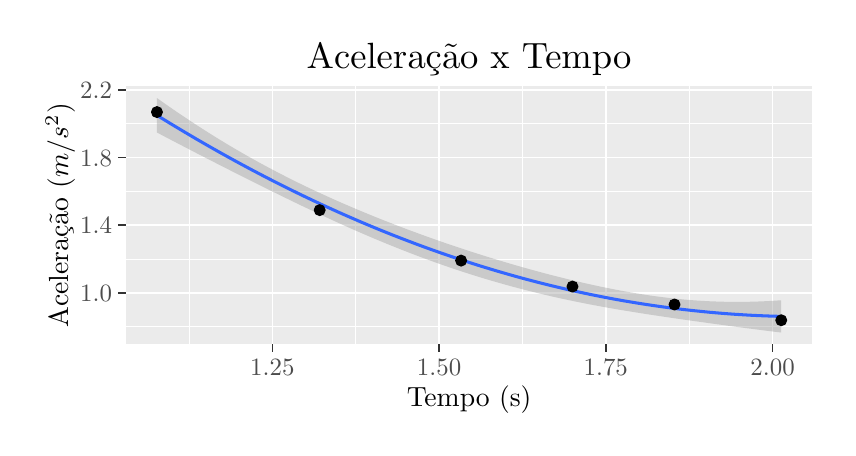
\begin{tikzpicture}[x=1pt,y=1pt]
\definecolor{fillColor}{RGB}{255,255,255}
\path[use as bounding box,fill=fillColor,fill opacity=0.00] (0,0) rectangle (289.08,144.54);
\begin{scope}
\path[clip] (  0.00,  0.00) rectangle (289.08,144.54);
\definecolor{drawColor}{RGB}{255,255,255}
\definecolor{fillColor}{RGB}{255,255,255}

\path[draw=drawColor,line width= 0.6pt,line join=round,line cap=round,fill=fillColor] (  0.00, -0.00) rectangle (289.08,144.54);
\end{scope}
\begin{scope}
\path[clip] ( 35.43, 30.14) rectangle (283.58,123.35);
\definecolor{fillColor}{gray}{0.92}

\path[fill=fillColor] ( 35.43, 30.14) rectangle (283.58,123.35);
\definecolor{drawColor}{RGB}{255,255,255}

\path[draw=drawColor,line width= 0.3pt,line join=round] ( 35.43, 36.43) --
	(283.58, 36.43);

\path[draw=drawColor,line width= 0.3pt,line join=round] ( 35.43, 60.89) --
	(283.58, 60.89);

\path[draw=drawColor,line width= 0.3pt,line join=round] ( 35.43, 85.35) --
	(283.58, 85.35);

\path[draw=drawColor,line width= 0.3pt,line join=round] ( 35.43,109.81) --
	(283.58,109.81);

\path[draw=drawColor,line width= 0.3pt,line join=round] ( 58.28, 30.14) --
	( 58.28,123.35);

\path[draw=drawColor,line width= 0.3pt,line join=round] (118.54, 30.14) --
	(118.54,123.35);

\path[draw=drawColor,line width= 0.3pt,line join=round] (178.79, 30.14) --
	(178.79,123.35);

\path[draw=drawColor,line width= 0.3pt,line join=round] (239.04, 30.14) --
	(239.04,123.35);

\path[draw=drawColor,line width= 0.6pt,line join=round] ( 35.43, 48.66) --
	(283.58, 48.66);

\path[draw=drawColor,line width= 0.6pt,line join=round] ( 35.43, 73.12) --
	(283.58, 73.12);

\path[draw=drawColor,line width= 0.6pt,line join=round] ( 35.43, 97.58) --
	(283.58, 97.58);

\path[draw=drawColor,line width= 0.6pt,line join=round] ( 35.43,122.04) --
	(283.58,122.04);

\path[draw=drawColor,line width= 0.6pt,line join=round] ( 88.41, 30.14) --
	( 88.41,123.35);

\path[draw=drawColor,line width= 0.6pt,line join=round] (148.66, 30.14) --
	(148.66,123.35);

\path[draw=drawColor,line width= 0.6pt,line join=round] (208.91, 30.14) --
	(208.91,123.35);

\path[draw=drawColor,line width= 0.6pt,line join=round] (269.17, 30.14) --
	(269.17,123.35);
\definecolor{fillColor}{RGB}{153,153,153}

\path[fill=fillColor,fill opacity=0.40] ( 46.71,119.11) --
	( 49.57,117.09) --
	( 52.42,115.11) --
	( 55.28,113.16) --
	( 58.14,111.25) --
	( 60.99,109.38) --
	( 63.85,107.54) --
	( 66.70,105.74) --
	( 69.56,103.97) --
	( 72.41,102.25) --
	( 75.27,100.56) --
	( 78.12, 98.91) --
	( 80.98, 97.29) --
	( 83.84, 95.71) --
	( 86.69, 94.17) --
	( 89.55, 92.66) --
	( 92.40, 91.19) --
	( 95.26, 89.74) --
	( 98.11, 88.33) --
	(100.97, 86.95) --
	(103.82, 85.60) --
	(106.68, 84.28) --
	(109.54, 82.98) --
	(112.39, 81.71) --
	(115.25, 80.47) --
	(118.10, 79.25) --
	(120.96, 78.05) --
	(123.81, 76.88) --
	(126.67, 75.72) --
	(129.52, 74.59) --
	(132.38, 73.48) --
	(135.24, 72.38) --
	(138.09, 71.31) --
	(140.95, 70.26) --
	(143.80, 69.22) --
	(146.66, 68.20) --
	(149.51, 67.20) --
	(152.37, 66.22) --
	(155.22, 65.26) --
	(158.08, 64.31) --
	(160.93, 63.38) --
	(163.79, 62.47) --
	(166.65, 61.58) --
	(169.50, 60.70) --
	(172.36, 59.85) --
	(175.21, 59.01) --
	(178.07, 58.18) --
	(180.92, 57.38) --
	(183.78, 56.60) --
	(186.63, 55.83) --
	(189.49, 55.08) --
	(192.35, 54.36) --
	(195.20, 53.65) --
	(198.06, 52.97) --
	(200.91, 52.31) --
	(203.77, 51.67) --
	(206.62, 51.05) --
	(209.48, 50.46) --
	(212.33, 49.90) --
	(215.19, 49.36) --
	(218.05, 48.86) --
	(220.90, 48.38) --
	(223.76, 47.93) --
	(226.61, 47.52) --
	(229.47, 47.15) --
	(232.32, 46.80) --
	(235.18, 46.50) --
	(238.03, 46.23) --
	(240.89, 46.01) --
	(243.75, 45.82) --
	(246.60, 45.67) --
	(249.46, 45.56) --
	(252.31, 45.48) --
	(255.17, 45.45) --
	(258.02, 45.46) --
	(260.88, 45.50) --
	(263.73, 45.58) --
	(266.59, 45.70) --
	(269.45, 45.85) --
	(272.30, 46.04) --
	(272.30, 34.37) --
	(269.45, 34.72) --
	(266.59, 35.08) --
	(263.73, 35.44) --
	(260.88, 35.81) --
	(258.02, 36.18) --
	(255.17, 36.56) --
	(252.31, 36.94) --
	(249.46, 37.33) --
	(246.60, 37.72) --
	(243.75, 38.12) --
	(240.89, 38.51) --
	(238.03, 38.92) --
	(235.18, 39.33) --
	(232.32, 39.74) --
	(229.47, 40.16) --
	(226.61, 40.59) --
	(223.76, 41.02) --
	(220.90, 41.47) --
	(218.05, 41.93) --
	(215.19, 42.40) --
	(212.33, 42.88) --
	(209.48, 43.38) --
	(206.62, 43.90) --
	(203.77, 44.43) --
	(200.91, 44.99) --
	(198.06, 45.56) --
	(195.20, 46.16) --
	(192.35, 46.77) --
	(189.49, 47.41) --
	(186.63, 48.08) --
	(183.78, 48.76) --
	(180.92, 49.47) --
	(178.07, 50.21) --
	(175.21, 50.96) --
	(172.36, 51.75) --
	(169.50, 52.56) --
	(166.65, 53.39) --
	(163.79, 54.25) --
	(160.93, 55.14) --
	(158.08, 56.05) --
	(155.22, 56.99) --
	(152.37, 57.95) --
	(149.51, 58.94) --
	(146.66, 59.95) --
	(143.80, 60.99) --
	(140.95, 62.05) --
	(138.09, 63.14) --
	(135.24, 64.25) --
	(132.38, 65.39) --
	(129.52, 66.55) --
	(126.67, 67.73) --
	(123.81, 68.93) --
	(120.96, 70.16) --
	(118.10, 71.40) --
	(115.25, 72.67) --
	(112.39, 73.95) --
	(109.54, 75.26) --
	(106.68, 76.58) --
	(103.82, 77.92) --
	(100.97, 79.27) --
	( 98.11, 80.63) --
	( 95.26, 82.01) --
	( 92.40, 83.40) --
	( 89.55, 84.80) --
	( 86.69, 86.21) --
	( 83.84, 87.63) --
	( 80.98, 89.05) --
	( 78.12, 90.49) --
	( 75.27, 91.93) --
	( 72.41, 93.37) --
	( 69.56, 94.82) --
	( 66.70, 96.28) --
	( 63.85, 97.74) --
	( 60.99, 99.21) --
	( 58.14,100.69) --
	( 55.28,102.17) --
	( 52.42,103.66) --
	( 49.57,105.15) --
	( 46.71,106.66) --
	cycle;
\definecolor{drawColor}{RGB}{51,102,255}

\path[draw=drawColor,line width= 1.1pt,line join=round] ( 46.71,112.88) --
	( 49.57,111.12) --
	( 52.42,109.38) --
	( 55.28,107.67) --
	( 58.14,105.97) --
	( 60.99,104.29) --
	( 63.85,102.64) --
	( 66.70,101.01) --
	( 69.56, 99.40) --
	( 72.41, 97.81) --
	( 75.27, 96.24) --
	( 78.12, 94.70) --
	( 80.98, 93.17) --
	( 83.84, 91.67) --
	( 86.69, 90.19) --
	( 89.55, 88.73) --
	( 92.40, 87.29) --
	( 95.26, 85.88) --
	( 98.11, 84.48) --
	(100.97, 83.11) --
	(103.82, 81.76) --
	(106.68, 80.43) --
	(109.54, 79.12) --
	(112.39, 77.83) --
	(115.25, 76.57) --
	(118.10, 75.33) --
	(120.96, 74.10) --
	(123.81, 72.90) --
	(126.67, 71.72) --
	(129.52, 70.57) --
	(132.38, 69.43) --
	(135.24, 68.32) --
	(138.09, 67.23) --
	(140.95, 66.15) --
	(143.80, 65.10) --
	(146.66, 64.08) --
	(149.51, 63.07) --
	(152.37, 62.09) --
	(155.22, 61.12) --
	(158.08, 60.18) --
	(160.93, 59.26) --
	(163.79, 58.36) --
	(166.65, 57.49) --
	(169.50, 56.63) --
	(172.36, 55.80) --
	(175.21, 54.99) --
	(178.07, 54.19) --
	(180.92, 53.43) --
	(183.78, 52.68) --
	(186.63, 51.95) --
	(189.49, 51.25) --
	(192.35, 50.57) --
	(195.20, 49.90) --
	(198.06, 49.26) --
	(200.91, 48.65) --
	(203.77, 48.05) --
	(206.62, 47.48) --
	(209.48, 46.92) --
	(212.33, 46.39) --
	(215.19, 45.88) --
	(218.05, 45.39) --
	(220.90, 44.93) --
	(223.76, 44.48) --
	(226.61, 44.06) --
	(229.47, 43.65) --
	(232.32, 43.27) --
	(235.18, 42.91) --
	(238.03, 42.58) --
	(240.89, 42.26) --
	(243.75, 41.97) --
	(246.60, 41.69) --
	(249.46, 41.44) --
	(252.31, 41.21) --
	(255.17, 41.00) --
	(258.02, 40.82) --
	(260.88, 40.65) --
	(263.73, 40.51) --
	(266.59, 40.39) --
	(269.45, 40.29) --
	(272.30, 40.21);
\definecolor{drawColor}{RGB}{0,0,0}
\definecolor{fillColor}{RGB}{0,0,0}

\path[draw=drawColor,line width= 0.4pt,line join=round,line cap=round,fill=fillColor] ( 46.71,114.04) circle (  1.96);

\path[draw=drawColor,line width= 0.4pt,line join=round,line cap=round,fill=fillColor] (105.52, 78.62) circle (  1.96);

\path[draw=drawColor,line width= 0.4pt,line join=round,line cap=round,fill=fillColor] (156.62, 60.37) circle (  1.96);

\path[draw=drawColor,line width= 0.4pt,line join=round,line cap=round,fill=fillColor] (196.86, 50.99) circle (  1.96);

\path[draw=drawColor,line width= 0.4pt,line join=round,line cap=round,fill=fillColor] (233.74, 44.50) circle (  1.96);

\path[draw=drawColor,line width= 0.4pt,line join=round,line cap=round,fill=fillColor] (272.30, 38.82) circle (  1.96);
\end{scope}
\begin{scope}
\path[clip] (  0.00,  0.00) rectangle (289.08,144.54);
\definecolor{drawColor}{gray}{0.30}

\node[text=drawColor,anchor=base east,inner sep=0pt, outer sep=0pt, scale=  0.90] at ( 30.48, 45.56) {1.0};

\node[text=drawColor,anchor=base east,inner sep=0pt, outer sep=0pt, scale=  0.90] at ( 30.48, 70.02) {1.4};

\node[text=drawColor,anchor=base east,inner sep=0pt, outer sep=0pt, scale=  0.90] at ( 30.48, 94.48) {1.8};

\node[text=drawColor,anchor=base east,inner sep=0pt, outer sep=0pt, scale=  0.90] at ( 30.48,118.94) {2.2};
\end{scope}
\begin{scope}
\path[clip] (  0.00,  0.00) rectangle (289.08,144.54);
\definecolor{drawColor}{gray}{0.20}

\path[draw=drawColor,line width= 0.6pt,line join=round] ( 32.68, 48.66) --
	( 35.43, 48.66);

\path[draw=drawColor,line width= 0.6pt,line join=round] ( 32.68, 73.12) --
	( 35.43, 73.12);

\path[draw=drawColor,line width= 0.6pt,line join=round] ( 32.68, 97.58) --
	( 35.43, 97.58);

\path[draw=drawColor,line width= 0.6pt,line join=round] ( 32.68,122.04) --
	( 35.43,122.04);
\end{scope}
\begin{scope}
\path[clip] (  0.00,  0.00) rectangle (289.08,144.54);
\definecolor{drawColor}{gray}{0.20}

\path[draw=drawColor,line width= 0.6pt,line join=round] ( 88.41, 27.39) --
	( 88.41, 30.14);

\path[draw=drawColor,line width= 0.6pt,line join=round] (148.66, 27.39) --
	(148.66, 30.14);

\path[draw=drawColor,line width= 0.6pt,line join=round] (208.91, 27.39) --
	(208.91, 30.14);

\path[draw=drawColor,line width= 0.6pt,line join=round] (269.17, 27.39) --
	(269.17, 30.14);
\end{scope}
\begin{scope}
\path[clip] (  0.00,  0.00) rectangle (289.08,144.54);
\definecolor{drawColor}{gray}{0.30}

\node[text=drawColor,anchor=base,inner sep=0pt, outer sep=0pt, scale=  0.90] at ( 88.41, 18.99) {1.25};

\node[text=drawColor,anchor=base,inner sep=0pt, outer sep=0pt, scale=  0.90] at (148.66, 18.99) {1.50};

\node[text=drawColor,anchor=base,inner sep=0pt, outer sep=0pt, scale=  0.90] at (208.91, 18.99) {1.75};

\node[text=drawColor,anchor=base,inner sep=0pt, outer sep=0pt, scale=  0.90] at (269.17, 18.99) {2.00};
\end{scope}
\begin{scope}
\path[clip] (  0.00,  0.00) rectangle (289.08,144.54);
\definecolor{drawColor}{RGB}{0,0,0}

\node[text=drawColor,anchor=base,inner sep=0pt, outer sep=0pt, scale=  1.00] at (159.51,  7.70) {Tempo (s)};
\end{scope}
\begin{scope}
\path[clip] (  0.00,  0.00) rectangle (289.08,144.54);
\definecolor{drawColor}{RGB}{0,0,0}

\node[text=drawColor,rotate= 90.00,anchor=base,inner sep=0pt, outer sep=0pt, scale=  1.00] at ( 14.59, 76.74) {Aceleração ($m/s^2$)};
\end{scope}
\begin{scope}
\path[clip] (  0.00,  0.00) rectangle (289.08,144.54);
\definecolor{drawColor}{RGB}{0,0,0}

\node[text=drawColor,anchor=base,inner sep=0pt, outer sep=0pt, scale=  1.32] at (159.51,129.95) {Aceleração x Tempo};
\end{scope}
\end{tikzpicture}
